% This version of CVPR template is provided by Ming-Ming Cheng.
% Please leave an issue if you found a bug:
% https://github.com/MCG-NKU/CVPR_Template.

% \documentclass[review]{cvpr}
\documentclass[final]{cvpr}

\usepackage{times}
\usepackage{epsfig}
\usepackage{graphicx}
\usepackage{amsmath}
\usepackage{amssymb}

% Include other packages here, before hyperref.

% If you comment hyperref and then uncomment it, you should delete
% egpaper.aux before re-running latex.  (Or just hit 'q' on the first latex
% run, let it finish, and you should be clear).
\usepackage[pagebackref=true,breaklinks=true,colorlinks,bookmarks=false]{hyperref}


\def\cvprPaperID{****} % *** Enter the CVPR Paper ID here
\def\confYear{CVPR 2021}
%\setcounter{page}{4321} % For final version only


\begin{document}

%%%%%%%%% TITLE
\title{Extraction of individual instrument sound from music file}

\author{Alex\\
student id\\
{\tt\small email}
% For a paper whose authors are all at the same institution,
% omit the following lines up until the closing ``}''.
% Additional authors and addresses can be added with ``\and'',
% just like the second author.
% To save space, use either the email address or home page, not both
\and
Teiichi\\
student id\\
{\tt\small email}
\and
Picard Armand\\
2021400607\\
{\tt\small armandpicard71@gmail.com}
}

\maketitle


%%%%%%%%% ABSTRACT
\begin{abstract}
Here is our abstract
\end{abstract}

%%%%%%%%% BODY TEXT
\section{Introduction}

Put introduction here

\section{Related work}

In this section we will describe different approche and model architecture to implements instrument sound extraction with DeepLearning.

\subsection{Different approches}
\subsubsection{Waveform}

This type of model take the raw wave as input

\subsubsection{Spectrogram}

Spectrogram model take the spectrogram of the audio as input.
To get the spectrogram, Short Time Fourier Transform(STFT) is use.
Then the DeepLearning model is given as input only the magnitude of the spectrogram and it train to produce the magnitude of the different source.
Then to get the final output we reintegrate the phase of the input signal and apply Inverse Short Time Fourier Transform(ISTFT) to get the output audio.

This approche allow the model to have higher level features as input and reduced lenght depending on the window size and the hop lenght while doing the STFT.
This higher level features can allow the model to learn faster and being smaller but it also don't give all the information on small local pertubation that can be usefull to produce the best final output.



\subsubsection{Hybrid}
The Hybrid approche use a network that have 2 input, one for the waveform and one for the spectrogram.
This allow to have the best of both world but require a lot of computing power. Example of this kind of model include HybridDemucs \cite{hybrid-demucs}

\subsection{Model architecture}

The main model architecture is based on UNet, this model use an encoder that downsample at each step and then a decoder that upsample the bottleneck using the result of each previous encoder as second input.
The global architecture of Wave-U-Net\cite{waveunet} is show in Figure~\ref{waveunet-architecture}

\begin{figure}
   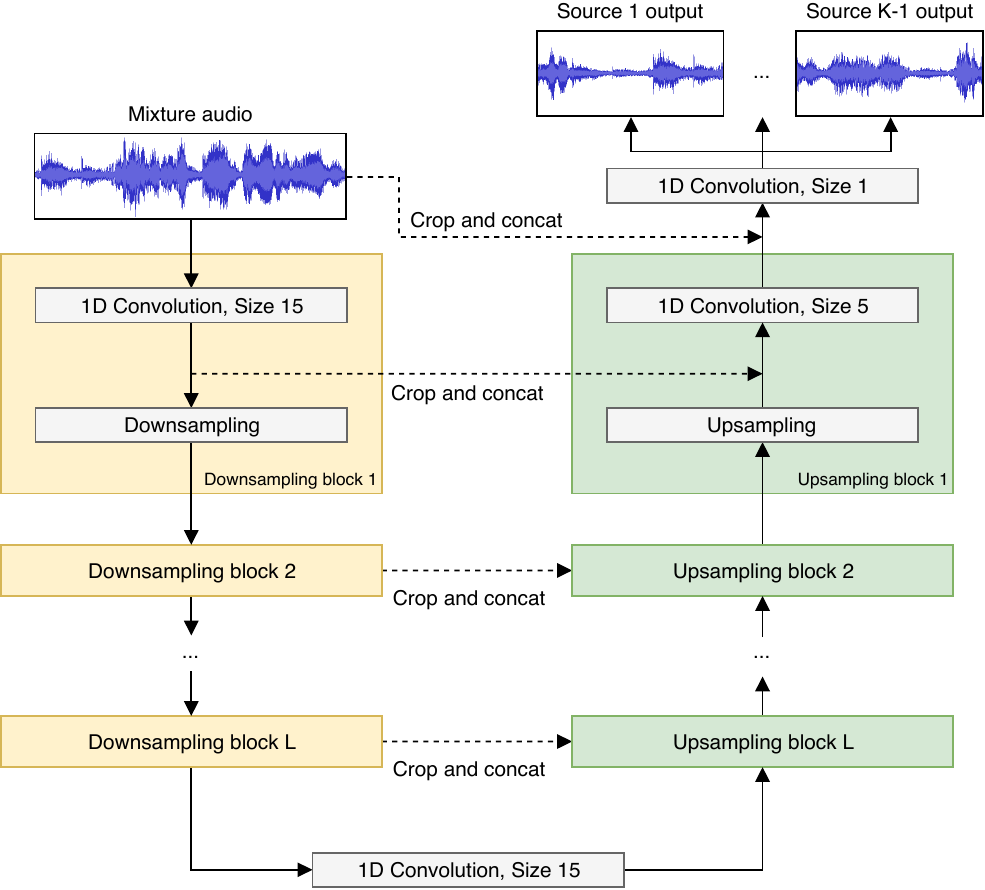
\includegraphics[scale=0.25]{waveunet.png}
   \caption{Wave-U-Net architecture}
   \label{waveunet-architecture}
\end{figure}

{\small
\bibliographystyle{ieee_fullname}
\bibliography{egbib}
}

\end{document}
